\chapter{Der Transformer} \label{Transformer}

In der zweiten Hälfte des Jahres 2017 ein Team von Wissenschaftlern veröffentlichte ihr Papier \textquotedblright Attention Is All You Need\textquotedblright, in dessen sie ein neues Model vorstellten. Das Projekt zur Entwicklung wurde unter der Google Research and Google Brain aufgeführt. Dieses Model nahm die Name der "Transformer".

\section{Struktur des Transformers}
Der Transformer besteht aus zwei Haupteinheiten, deren Namen Encoder und Decoder sind. Die beiden Einheiten bestehen aus gleicher Anzahl Encoder-, bzw. Decoder-, Layers. Der im Pappier vorgestellte Encoder verfügte über 6 Encoderschichten und 6 Decoderschichten. Die folgende Abbildung beschreibt den Transformer:


\begin{figure}
	\centering
	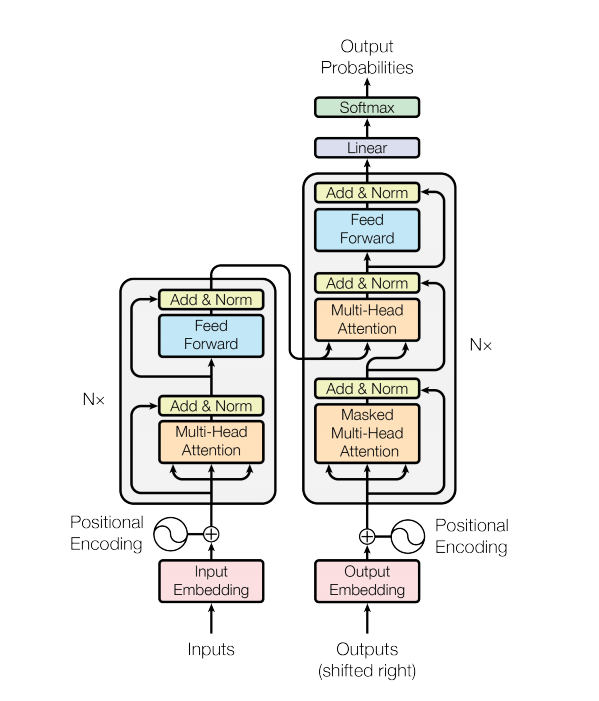
\includegraphics[scale=0.36]{images/transformer.png}
	\caption{Das Transformer-Modell}
	\label{transformer}
\end{figure}

In den linken Schichten fließt der Input, meistens mehrere Sätze, durch eine Attention- und eine FeedForward-Network(FFN) Unterschicht. Rechts werden die Targeteingaben, die zugehörigen Sätze für den Input, von zwei Attention- und wieder von einer FFN-Unterschichten. Der Input- und der Targetsatz werden eingebettet, before sie in den Encoder, bzw. Decoder, eingegeben worden. Zuerst werden die einzelnen Wörter der Sätze durch ihre entsprechende Kodierung in Zahlen ersetzt. Demnächst wird eine Positionale Kodierung in der Eingabe eingebettet.

Die nächsten Unterkapitel betrachten die einzelnen Aufbauelementen des Transformers ins Details. Wichtig ist es Hier zu erwähnen, dass die Positionale Einbettung von keiner Einheit im Transformer durchgeführt ist, sondern eine zusätzliche Vorbearbeitung des Textes (Text Preprocessing). Jedoch erkläre ich die Mathematik, die dahinter steckt.

\subsection{Positionale Einbettung}
Die Positionale Einbettung passiert nach der Umwandlung von Text in Zahlen. Wie die Name erratet, wird Information über die Lage des Wortes im Satz in den Wortvektor eingebettet. Diese zusätliche Aktion ist notwig, da im vergleich zu anderen Modelle oder Verfahren, beihaltet der Transformer keine Convolutional- oder Recurenz-Netzwerke.

Die Formel nach dem der Vektor berechnet wird, ist gegeben:

\begin{equation}
	PE_{(pos,2i)} = \sin\Bigg(\frac{pos}{10000^\frac{2i}{d_{model}}}\Bigg)
\end{equation}
\begin{equation}
	PE_{(pos,2i+1)} = \cos\Bigg(\frac{pos}{10000^\frac{2i}{d_{model}}}\Bigg)
\end{equation}

Der PE-Vektor besteht aus $d_model$-Dimensionen. Für jede Dimension wird der Wert des Eintrages entweder mit der Sinus oder der Cosinus-Funktion berechnet. Die geraden Dimensionen entsprechend mit der Sinusfunktion und die Ungeraden mit der Cosinusfunktion.

Als nächstes wird betrachtet, wie der PE-Vektor zum Einbettungs-Vektor addiert wird. In der Literatur werden die Vektoren ganz einfache addiert. Diese Vorgehensweise könnte jedoch Probleme verursachen und wichtige Informationen könnten verloren gehen. Es existieren mehrere Möglichkeiten, wie man das Verlust von Informationen zu vermeiden. Im Buch \cite{denis_Transformer:02} wird folgende Formel benutzt:

\begin{equation}
	pc(i) = y_i*math.sqrt(d_{model}) + pe(i)
\end{equation}

,wo der Eingabevektor durch eine Konstante skaliert wird. Die Variable $y_i$ ist der eingebettete Vektor und $pe$ ist der Positionalsvektor und $d_{model}$ entspricht die Anzahl der Dimensionen des Vektoren benutzt im Model. Der Eingabevektor wird mit dem Wurzel vom Dimensionen skaliert und erst dann wird der Positionalvektor addiert.

\subsection{Encoder und Decoder}

Encoder und Decoder sind die essenziellen Bestandteile vom Transformer. Der Encoder erhält die schon veränderten Daten und führt sie durch ein Attention- und ein Feed Forward Network-Layer. Zwischen jeder Unterschicht besteht eine residierte Verbindung (siehe Abbildung \ref{transformer}), sodass die Ausgaben vom letzten Unterlayer mit den Ausgaben vom Aktuellen addiert und weiterhin normiert werden. Der Decoder besitzt eine Unterschicht mehr als der Encoder. In der Transformer beinhaltet der Decoder drei Schichten (siehe Abbildung \ref{transformer}). Die letzten zwei sind die selben wie im Encoder. Die erste Unterschicht im Decoder ist eine Masked-Multi-Head-Attention-Schicht. Die Verbindung zwischen Encoder und Decoder erfolgt in der zweiten Unterschicht - zwar in der MHA-Schicht. Da werden die Ausgaben vom Encoder und vom MMHA-Schicht zusammengeführt. Nach der Bearbeitung liefert das Model einen potenziellen Satz, der abhängig vom Aufgaben Stellung, die gesuchte Antwort sein sollte. In diesem Fall ist es die Übersetzung aus dem Englishen ins Spanische. In den folgenden Unterkapiteln werden die Unterschichten ins Details untersucht.

\subsubsection{Multi-Head-Attention Layer}
Der Multi-Head-Attention Layer kommt in den beiden Einheiten vor. Dieser Schicht folgt eine Normierungsschicht, die die Ausgaben aus dem MHA-Schicht und die Residial-Daten aus vorheriger Schicht addiert und normiert.

Die Eingabe in dem Multi-Head-Attention-Layer vom Encoder ist der Vektor, der die positionale und eingebettete Angaben vom Text erhählt. Im Decoder erhält der MHA-Layer die Eingaben von einer Masked-Multi-Head-Attention-Schicht, und somit ist die Information bis zum aktuell betrachteten Punkt. Der unteschied besteht darin, dass die Information für den Encoder komplett verfügbar ist, und im Decoder wird diese maskiert, und so lernt das Model zu raten. Darin besteht der Unterschied zwischen den MHA im Encoder und Decoder. 

Ziel dem MHA-Layer im Encoder` ist es die Bezihung zwischen einzelnen Worten zu bestimmen. Das wird erzielt, indem jedes Wort aus dem Satz mit allen anderen abgebildet wird. Jedoch  Jedes Wortvektor besteht aus $d_{model}$ Dimensionen. In dem Buch \cite{denis_Transformer:02} entspricht die Anzahl an Dimensionen gleich 512. Die große Anzahl der Dimensionen würde große Laufzeit anfordern, wenn mehrere Ansichten untersucht werden wollen. Dies ist natürlich möglich mit den stärken Komputern von heute. Der Nachteil ist natürlich, dass das Model immer nur eine Ansicht über die Beziehungen der Wörter betrachtet und es natürlich noch mehr Leistung erfordern würde, um weitere Ansichten zu bestimmen. Eine bessere Alternative ist die Dimensionen jedes Wortes in 8 Teilen, jedem Teil (auch Head genannt im \cite{denis_Transformer:02}) entspricht 64 Dimensionen, aufzuteilen. Dann wird jeder 64-stückige Teil den 8 unterschiedlichen Heads (deswegen ist die Schicht Multi-Head-Attention-Layer genannt; siehe Abbildung \ref{multi_head}) zum untersuchen gegeben. 

\begin{figure}
	\centering
	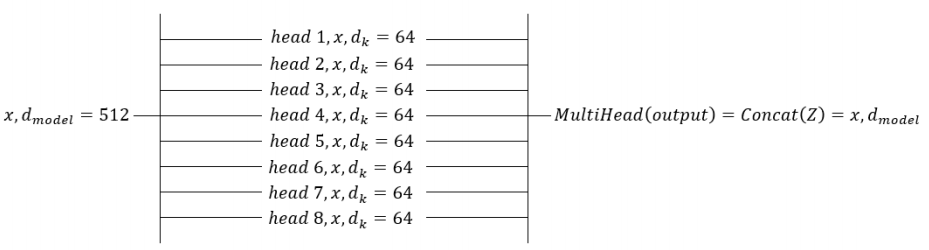
\includegraphics[scale=0.4]{images/multi_head.png}
	\caption{Heads \cite{denis_Transformer:02}}
	\label{multi_head}
\end{figure}

Diese ``Köpfe'' laufen parallel. Der Vorteil dabei ist es, dass die Laufzeit verringert wird und es 8 unterschiedliche Repräsentationen betrachtet werden. In der Abbildung \ref{multi_head} erkennt man wie die MHA-Schicht aussieht. Nachdem die Daten von jedem Kopf vorhanden sind, werden die Ergebnisvektoren wieder konkateniert (siehe Abbildung \ref{multi_head}). Die Ausgabe sieht, dann wie folgt aus:

\begin{equation}
	Z = (z_0, z_1, z_2, z_3, z_4, z_5, z_6, z_7)
\end{equation}

Die Matrix Z ist die aus den Ausgaben $z_i$ aufgebaute Ergebnismatrix. Am Ende muss die Matrix $Z$ zusätzlich konkateniert werden, um die ursprünglichen Dimensionen $x*d_{model}$ zu erhalten.

In jedem Kopf wird jedes Wort mit drei Vektoren repräsentiert:
\begin{itemize}
	\item Einem Query-Vektor ($Q$), dessen Dimensionalität $d_q$ gleich \textbf{64} ist. Der Vektor wird verwendet, oder trainiert, wenn der zugehörige Wortvektor für $x_n$ die Key-Value-Paare gesucht sind, inklusive sich selbst.
	
	\item Einem Schlüsselvektor (auch als Key-Vektor bezeichnet $K$), der trainiert wird, um einen Attention-Wert zu ergeben.
	
	\item Einem Wertvektor (auch als Value-Vektor bezeichnet $V$), der trainiert wird, um einen weitere Anttention-Wert zu ergeben.
\end{itemize}

Im Buch \cite{denis_Transformer:02} wird das Attention als "Scaled Dot-Product Attention" bezeichnet. Das ist eine Linearkombination der oben deklarierten Vektoren. Die folgende Formel ergibt seine Berechnung: 

\begin{equation}
	Attention(Q, K, V) = softmax\Bigg(\frac{Q*K^T}{\sqrt{d_k}}\Bigg)* V
\end{equation}

Diese Vektorrepräsentationen werden aus den Gewichtsmatrizen eingelesen. Die Gewichtsmatrizen, sind am Anfang nicht bekannt und werden im Folge der Training bestimmt. Zu Beginn werden sie mit zufälligen Werten erstellt. Die Matrizen werden im Buch \cite{denis_Transformer:02} als $Q_w$, $K_w$ und $V_k$ beschriftet. Sie besitzen $d_k$ = \textbf{64} Spalten und $d_model$ = \textbf{512} Zeilen. Wenn zum Beispiel ein bestimmtes Query für den Wort $x_n$ abzulesen ist, dann erfolgt das durch eine einfache Matrixmultiplikation:

\begin{equation}
	Q_{x_n} = x_n * Q_w
	K_{x_n} = x_n * K_w
	V_{x_n} = x_n * V_w
\end{equation}

Wobei $x_n$ repräsentiert in diesem Fall den Indexwert vom Wort $x_n$. Wenn die Eingabe aus mehreren Worten besteht, wird eine Matrix mit den Dimensionen Anzahl der Worte*$d_{model}$ (für $d_{model}$ meistens 512 gewählt) erhalten.

Für jeden Eintrag in x wird eine Matrix mit seinen Attention-Vektoren berechnet, bzw. den Beziehungsvektoren zu jedem Eingabewort $x_n$ (inklusive sich selbst). Jeder Vektor in der Matrix hat 512 Einträge, und es gibt insgesammt $m$-viele Vektoren ($m-viele$ Wörter). Den Attention-Vektor für jedes Wort wird erhalten, indem die Vektoren aus der Matrix summiert werden. Schließlich wird jedes Attention-Vektor von allen Heads zusammengeführt, und diese bauen die Attention-Matrix auf. Eine Normierungsschicht folgt der Attnetion-Schicht. Die erhält als Eingabe die konkatenierte Ausgabe Matrix $Z_{concant}$ und die unveränderten Eingabedaten der MHA-Attentionschicht $x$:

\begin{equation}
	v = x + Z_{concat}.
\end{equation}
Die Normierungsschicht führt folgende Berehcnungen dann aus:

\begin{equation}
	LayerNorm(v) = \gamma * \frac{v - \mu}{\delta} + \beta.
\end{equation}
Die Veraiblen bedeuten folgendes:

\begin{itemize}[leftmargin=1cm]
		\item $\mu$ ist der Durchschnitt von $v$ mit Dimensionen d:
		\begin{equation}
			\mu = \frac{1}{d}\sum_{k=1}^{d} v_k.
		\end{equation}
		\item $\delta$ ist die Standardabweichung von $v$ mit Dimensionen d:
		\begin{equation}
			delta^2 = \frac{1}{d}\sum_{d}^{k=1} (v_k - \mu)^2.
		\end{equation}
		\item $\gamma$ ist ein Skalierungsparameter.
		\item $\beta$ ist ein Bias-Vektor.
\end{itemize}

Die weiteren Normierungsschichten im Modell führen analoge Operationen und diese Erläuterung dient als Muster für die weiteren. Somit werden alle anderen Normierungsschichten nicht betrachtet.

Analog sieht die Funktionalität der MHA-Schicht im Decoder aus. Die Eingabe im der Schicht erfolgt aus dem Masked-Multi-Head-Attention-Layer und der Ausgabe des Encoders. Als nächstes wird der Feed-Forward-Network-Sublayer erläutert.

\subsubsection{Feed Forward Network}

Die Eingabe im Feed-Forward-Network ist die Ausgabe der Normierungsschicht (siehe Abbildung \ref{transformer}). Die Eingabe ist ein $d_{model}$ Dimensionales Vektor. Die Struktur des FFN-Layers kann wie folgt beschrieben werden \cite{Vaswani:2017}:

\begin{itemize}[leftmargin=1cm]
	\item Die Schichten sind sowohl im Encoder als auch im Decoder komplett verbunden.
	
	\item Die FFN ist für jeder Wort einzeln anzuwenden. Die Anwendung ist indentisch, jedoch mit unterschiedlichen Parametern.
	
	\item Der Netzwerk besteht aus zwei Lienearetransformationen und eine ReLU-Aktivation dazwischen:
	\begin{equation}
		FFN(x) = max(0, x*W_1 + b_1)*W_2 + b_2.
	\end{equation}
	
	\item Die Ein- und Ausgabe des FFN haben eine Dimensionalität von $d_model$ = 512. Die innere Schicht besteht aus $d_{ff}$	= 2048 Neuronen.
\end{itemize}

Sowohl im Encoder als auch im Decoder ist die Struktur und Funktionalität der FFN-Schicht gleich. Die Ausgaben der FFN-Schicht werden wieder normiert. Die Inputdaten von der nachfolgenden Normierungsschicht sind die Ausgabe vom FFN und dessen Eingabe (in beiden Einheiten gleich; siehe Abbildung \ref{transformer}).


\subsubsection{Masked Multi-Head Attention Layer}

Die letzte Schicht vom Decoder ist die Masked-Multi-Head-Attentnion-Schicht. Diese Schicht hat den selben Aufbau wie die MHA-Schicht. Diese Schicht unterscheidet sich von der im Encoder darin, dass die Eingabe  ``maskiert'' wird. Das bedeutet, dass bestimmte Abschnitte maskiert werden, sodass der Layer begrenzte Informationen erhält. Ziel der Maskierung ist es dem Model zu zwingen, die unbekannten Stellen zu Raten. Deswegen betrachtet das Netz die Information nur bis zur aktuellen Position und die nachfolgenden Stellen müssen erraten werden.

\section{Implementierung}

Die Implementierung des Transformers ist sehr komplex. Der Programmcode kann außerdem auf der Tensorflow Seite \cite{transformer_tensorflow:21} gefunden werden. 

\subsubsection{Die Klasse}
Für den Aufbau des Models werden 6 Klassen Gebraucht. Diese sechs Klassen beschreiben die wichtigsten Komponente des Transformers und das Model selbst. Es gibt zwei Klassen für den Encoder und Decoder, zwei für die Layers im Encoder und Decoder, die Klasse für das Model und eine Klasse für den Attentionlayers. Zur besseren Überblick stelle ich die Hauptklasse des Transformers:

\begin{lstlisting}[language=Python, caption={Definition des Transformers}]
self.encoder = Encoder(num_layers, d_model, num_heads, dff, input_vocab_size, pe_input, rate)
self.decoder = Decoder(num_layers, d_model, num_heads, dff, target_vocab_size, pe_target)
self.dense = Dense(target_vocab_size)
\end{lstlisting}

Die Codezeilen sprechen für sich selbst. Die Dense-Schicht repräsentiert einen komplett verbundenen Netzwerk mit \textit{target\_vocab\_size}-viele Neuronen. Die Ausgabe davon entspricht die Schätzung des Models. Für jeden einzelnen Wort im Satz wird der Decoded-Vektor in einem anderen Vektor mit Dimensionalität \textit{sequence\_length} $\times$ \textit{target\_vocab\_size} verwandelt. Für jede Stelle im Satz liefert die Denseschicht einen Vektor, der so Groß ist wie die Anzahl der einzigartige Wörter im Targetcorpus, mit den Wahrscheinlichkeiten, dass das Wort an der Stelle platziert werden soll. Somit ratet das Model. Der Encoder und Decoder werden mit den bestimmten Hyperparametern inizialisiert. In meinem Fall verwende ich einen Transformer mit folgenden Hyperparametern:

\begin{lstlisting}[language=Python, caption={Hyperparameter}]
num_layers = 6
d_model = 512
dff = 2048
num_heads = 8
\end{lstlisting}

Diese Variablen haben die selben Werte wie der ursprüngliche Transformer \cite{Vaswani:2017}.

\subsubsection{Encoder}

Die Encoder Klasse besteht aus mehreren Encoderschichten und die entsprechende Embeddingschicht. Die Klasse sieht wie folgt aus:

\begin{lstlisting}[language=Python, caption={Encoder}]
self.embedding = Embedding(input_vocab_size, d_model)
self.pos_encoding = self.positional_encoding(maximum_position_encoding, self.d_model)
self.enc_layers = [EncoderLayer(d_model, num_heads, dff, rate) for _ in range(self.num_layers)]
self.dropout = Dropout(rate)
\end{lstlisting}

Hier erkennt man die zwei Einbettungsschichten, eine für die Tokeneinbettung und die zweite für die Positionaleeinbettung. In der dritte Zeile werden alle Encoderschichten erstellt. Am Ende wird ein Dropoutschicht angehängt, der dabei Hilft, das Model nicht übertreniert (overfitting) zu werden.

\subsubsection{Decoder}



